\documentclass[1p]{elsarticle_modified}
%\bibliographystyle{elsarticle-num}

%\usepackage[colorlinks]{hyperref}
%\usepackage{abbrmath_seonhwa} %\Abb, \Ascr, \Acal ,\Abf, \Afrak
\usepackage{amsfonts}
\usepackage{amssymb}
\usepackage{amsmath}
\usepackage{amsthm}
\usepackage{scalefnt}
\usepackage{amsbsy}
\usepackage{kotex}
\usepackage{caption}
\usepackage{subfig}
\usepackage{color}
\usepackage{graphicx}
\usepackage{xcolor} %% white, black, red, green, blue, cyan, magenta, yellow
\usepackage{float}
\usepackage{setspace}
\usepackage{hyperref}

\usepackage{tikz}
\usetikzlibrary{arrows}

\usepackage{multirow}
\usepackage{array} % fixed length table
\usepackage{hhline}

%%%%%%%%%%%%%%%%%%%%%
\makeatletter
\renewcommand*\env@matrix[1][\arraystretch]{%
	\edef\arraystretch{#1}%
	\hskip -\arraycolsep
	\let\@ifnextchar\new@ifnextchar
	\array{*\c@MaxMatrixCols c}}
\makeatother %https://tex.stackexchange.com/questions/14071/how-can-i-increase-the-line-spacing-in-a-matrix
%%%%%%%%%%%%%%%

\usepackage[normalem]{ulem}

\newcommand{\msout}[1]{\ifmmode\text{\sout{\ensuremath{#1}}}\else\sout{#1}\fi}
%SOURCE: \msout is \stkout macro in https://tex.stackexchange.com/questions/20609/strikeout-in-math-mode

\newcommand{\cancel}[1]{
	\ifmmode
	{\color{red}\msout{#1}}
	\else
	{\color{red}\sout{#1}}
	\fi
}

\newcommand{\add}[1]{
	{\color{blue}\uwave{#1}}
}

\newcommand{\replace}[2]{
	\ifmmode
	{\color{red}\msout{#1}}{\color{blue}\uwave{#2}}
	\else
	{\color{red}\sout{#1}}{\color{blue}\uwave{#2}}
	\fi
}

\newcommand{\Sol}{\mathcal{S}} %segment
\newcommand{\D}{D} %diagram
\newcommand{\A}{\mathcal{A}} %arc


%%%%%%%%%%%%%%%%%%%%%%%%%%%%%5 test

\def\sl{\operatorname{\textup{SL}}(2,\Cbb)}
\def\psl{\operatorname{\textup{PSL}}(2,\Cbb)}
\def\quan{\mkern 1mu \triangleright \mkern 1mu}

\theoremstyle{definition}
\newtheorem{thm}{Theorem}[section]
\newtheorem{prop}[thm]{Proposition}
\newtheorem{lem}[thm]{Lemma}
\newtheorem{ques}[thm]{Question}
\newtheorem{cor}[thm]{Corollary}
\newtheorem{defn}[thm]{Definition}
\newtheorem{exam}[thm]{Example}
\newtheorem{rmk}[thm]{Remark}
\newtheorem{alg}[thm]{Algorithm}

\newcommand{\I}{\sqrt{-1}}
\begin{document}

%\begin{frontmatter}
%
%\title{Boundary parabolic representations of knots up to 8 crossings}
%
%%% Group authors per affiliation:
%\author{Yunhi Cho} 
%\address{Department of Mathematics, University of Seoul, Seoul, Korea}
%\ead{yhcho@uos.ac.kr}
%
%
%\author{Seonhwa Kim} %\fnref{s_kim}}
%\address{Center for Geometry and Physics, Institute for Basic Science, Pohang, 37673, Korea}
%\ead{ryeona17@ibs.re.kr}
%
%\author{Hyuk Kim}
%\address{Department of Mathematical Sciences, Seoul National University, Seoul 08826, Korea}
%\ead{hyukkim@snu.ac.kr}
%
%\author{Seokbeom Yoon}
%\address{Department of Mathematical Sciences, Seoul National University, Seoul, 08826,  Korea}
%\ead{sbyoon15@snu.ac.kr}
%
%\begin{abstract}
%We find all boundary parabolic representation of knots up to 8 crossings.
%
%\end{abstract}
%\begin{keyword}
%    \MSC[2010] 57M25 
%\end{keyword}
%
%\end{frontmatter}

%\linenumbers
%\tableofcontents
%
\newcommand\colored[1]{\textcolor{white}{\rule[-0.35ex]{0.8em}{1.4ex}}\kern-0.8em\color{red} #1}%
%\newcommand\colored[1]{\textcolor{white}{ #1}\kern-2.17ex	\textcolor{white}{ #1}\kern-1.81ex	\textcolor{white}{ #1}\kern-2.15ex\color{red}#1	}

{\Large $\underline{11a_{341}~(K11a_{341})}$}

\setlength{\tabcolsep}{10pt}
\renewcommand{\arraystretch}{1.6}
\vspace{1cm}\begin{tabular}{m{100pt}>{\centering\arraybackslash}m{274pt}}
\multirow{5}{120pt}{
	\centering
	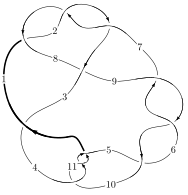
\includegraphics[width=112pt]{../../../GIT/diagram.site/Diagrams/png/590_11a_341.png}\\
\ \ \ A knot diagram\footnotemark}&
\allowdisplaybreaks
\textbf{Linearized knot diagam} \\
\cline{2-2}
 &
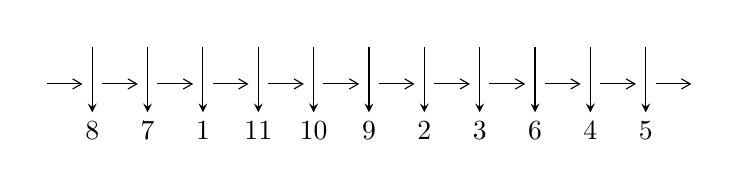
\begin{tikzpicture}[x=20pt, y=17pt]
	% nodes
	\node (C0) at (0, 0) {};
	\node (C1) at (1, 0) {};
	\node (C1U) at (1, +1) {};
	\node (C1D) at (1, -1) {8};

	\node (C2) at (2, 0) {};
	\node (C2U) at (2, +1) {};
	\node (C2D) at (2, -1) {7};

	\node (C3) at (3, 0) {};
	\node (C3U) at (3, +1) {};
	\node (C3D) at (3, -1) {1};

	\node (C4) at (4, 0) {};
	\node (C4U) at (4, +1) {};
	\node (C4D) at (4, -1) {11};

	\node (C5) at (5, 0) {};
	\node (C5U) at (5, +1) {};
	\node (C5D) at (5, -1) {10};

	\node (C6) at (6, 0) {};
	\node (C6U) at (6, +1) {};
	\node (C6D) at (6, -1) {9};

	\node (C7) at (7, 0) {};
	\node (C7U) at (7, +1) {};
	\node (C7D) at (7, -1) {2};

	\node (C8) at (8, 0) {};
	\node (C8U) at (8, +1) {};
	\node (C8D) at (8, -1) {3};

	\node (C9) at (9, 0) {};
	\node (C9U) at (9, +1) {};
	\node (C9D) at (9, -1) {6};

	\node (C10) at (10, 0) {};
	\node (C10U) at (10, +1) {};
	\node (C10D) at (10, -1) {4};

	\node (C11) at (11, 0) {};
	\node (C11U) at (11, +1) {};
	\node (C11D) at (11, -1) {5};
	\node (C12) at (12, 0) {};

	% arrows
	\draw[->,>={angle 60}]
	(C0) edge (C1) (C1) edge (C2) (C2) edge (C3) (C3) edge (C4) (C4) edge (C5) (C5) edge (C6) (C6) edge (C7) (C7) edge (C8) (C8) edge (C9) (C9) edge (C10) (C10) edge (C11) (C11) edge (C12) ;	\draw[->,>=stealth]
	(C1U) edge (C1D) (C2U) edge (C2D) (C3U) edge (C3D) (C4U) edge (C4D) (C5U) edge (C5D) (C6U) edge (C6D) (C7U) edge (C7D) (C8U) edge (C8D) (C9U) edge (C9D) (C10U) edge (C10D) (C11U) edge (C11D) ;
	\end{tikzpicture} \\
\hhline{~~} \\& 
\textbf{Solving Sequence} \\ \cline{2-2} 
 &
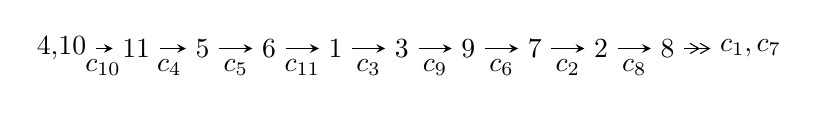
\begin{tikzpicture}[x=24pt, y=7pt]
	% node
	\node (A0) at (-1/8, 0) {4,10};
	\node (A1) at (1, 0) {11};
	\node (A2) at (2, 0) {5};
	\node (A3) at (3, 0) {6};
	\node (A4) at (4, 0) {1};
	\node (A5) at (5, 0) {3};
	\node (A6) at (6, 0) {9};
	\node (A7) at (7, 0) {7};
	\node (A8) at (8, 0) {2};
	\node (A9) at (9, 0) {8};
	\node (C1) at (1/2, -1) {$c_{10}$};
	\node (C2) at (3/2, -1) {$c_{4}$};
	\node (C3) at (5/2, -1) {$c_{5}$};
	\node (C4) at (7/2, -1) {$c_{11}$};
	\node (C5) at (9/2, -1) {$c_{3}$};
	\node (C6) at (11/2, -1) {$c_{9}$};
	\node (C7) at (13/2, -1) {$c_{6}$};
	\node (C8) at (15/2, -1) {$c_{2}$};
	\node (C9) at (17/2, -1) {$c_{8}$};
	\node (A10) at (41/4, 0) {$c_{1},c_{7}$};

	% edge
	\draw[->,>=stealth]	
	(A0) edge (A1) (A1) edge (A2) (A2) edge (A3) (A3) edge (A4) (A4) edge (A5) (A5) edge (A6) (A6) edge (A7) (A7) edge (A8) (A8) edge (A9) ;
	\draw[->>,>={angle 60}]	
	(A9) edge (A10);
\end{tikzpicture} \\ 

\end{tabular} \\

\footnotetext{
The image of knot diagram is generated by the software ``\textbf{Draw programme}" developed by Andrew Bartholomew(\url{http://www.layer8.co.uk/maths/draw/index.htm\#Running-draw}), where we modified some parts for our purpose(\url{https://github.com/CATsTAILs/LinksPainter}).
}\phantom \\ \newline 
\centering \textbf{Ideals for irreducible components\footnotemark of $X_{\text{par}}$} 
 
\begin{align*}
I^u_{1}&=\langle 
u^{30}- u^{29}+\cdots+u-1\rangle \\
\\
\end{align*}
\raggedright * 1 irreducible components of $\dim_{\mathbb{C}}=0$, with total 30 representations.\\
\footnotetext{All coefficients of polynomials are rational numbers. But the coefficients are sometimes approximated in decimal forms when there is not enough margin.}
\newpage
\renewcommand{\arraystretch}{1}
\centering \section*{I. $I^u_{1}= \langle u^{30}- u^{29}+\cdots+u-1 \rangle$}
\flushleft \textbf{(i) Arc colorings}\\
\begin{tabular}{m{7pt} m{180pt} m{7pt} m{180pt} }
\flushright $a_{4}=$&$\begin{pmatrix}0\\u\end{pmatrix}$ \\
\flushright $a_{10}=$&$\begin{pmatrix}1\\0\end{pmatrix}$ \\
\flushright $a_{11}=$&$\begin{pmatrix}1\\u^2\end{pmatrix}$ \\
\flushright $a_{5}=$&$\begin{pmatrix}- u\\- u^3+u\end{pmatrix}$ \\
\flushright $a_{6}=$&$\begin{pmatrix}u^3-2 u\\- u^3+u\end{pmatrix}$ \\
\flushright $a_{1}=$&$\begin{pmatrix}- u^2+1\\- u^4+2 u^2\end{pmatrix}$ \\
\flushright $a_{3}=$&$\begin{pmatrix}u^5-2 u^3+u\\u^7-3 u^5+2 u^3+u\end{pmatrix}$ \\
\flushright $a_{9}=$&$\begin{pmatrix}u^6-3 u^4+2 u^2+1\\- u^6+2 u^4- u^2\end{pmatrix}$ \\
\flushright $a_{7}=$&$\begin{pmatrix}u^9-4 u^7+5 u^5-3 u\\- u^9+3 u^7-3 u^5+u\end{pmatrix}$ \\
\flushright $a_{2}=$&$\begin{pmatrix}u^{25}-10 u^{23}+\cdots+10 u^3+u\\- u^{25}+9 u^{23}+\cdots-2 u^3+u\end{pmatrix}$ \\
\flushright $a_{8}=$&$\begin{pmatrix}- u^{18}+7 u^{16}-20 u^{14}+27 u^{12}-11 u^{10}-13 u^8+16 u^6-6 u^4+u^2+1\\- u^{20}+8 u^{18}-26 u^{16}+40 u^{14}-19 u^{12}-24 u^{10}+30 u^8-2 u^6-5 u^4-2 u^2\end{pmatrix}$\\ \flushright $a_{8}=$&$\begin{pmatrix}- u^{18}+7 u^{16}-20 u^{14}+27 u^{12}-11 u^{10}-13 u^8+16 u^6-6 u^4+u^2+1\\- u^{20}+8 u^{18}-26 u^{16}+40 u^{14}-19 u^{12}-24 u^{10}+30 u^8-2 u^6-5 u^4-2 u^2\end{pmatrix}$\\&\end{tabular}
\flushleft \textbf{(ii) Obstruction class $= -1$}\\~\\
\flushleft \textbf{(iii) Cusp Shapes $= 4 u^{27}-40 u^{25}-4 u^{24}+176 u^{23}+36 u^{22}-420 u^{21}-140 u^{20}+508 u^{19}+284 u^{18}-52 u^{17}-256 u^{16}-716 u^{15}-96 u^{14}+840 u^{13}+440 u^{12}-64 u^{11}-296 u^{10}-520 u^9-112 u^8+264 u^7+192 u^6+96 u^5-16 u^4-64 u^3-32 u^2-16 u-10$}\\~\\
\newpage\renewcommand{\arraystretch}{1}
\flushleft \textbf{(iv) u-Polynomials at the component}\newline \\
\begin{tabular}{m{50pt}|m{274pt}}
Crossings & \hspace{64pt}u-Polynomials at each crossing \\
\hline $$\begin{aligned}c_{1},c_{2},c_{7}\end{aligned}$$&$\begin{aligned}
&u^{30}- u^{29}+\cdots- u-1
\end{aligned}$\\
\hline $$\begin{aligned}c_{3},c_{5},c_{6}\\c_{9}\end{aligned}$$&$\begin{aligned}
&u^{30}-3 u^{29}+\cdots-7 u+3
\end{aligned}$\\
\hline $$\begin{aligned}c_{4},c_{10},c_{11}\end{aligned}$$&$\begin{aligned}
&u^{30}+u^{29}+\cdots- u-1
\end{aligned}$\\
\hline $$\begin{aligned}c_{8}\end{aligned}$$&$\begin{aligned}
&u^{30}+u^{29}+\cdots-135 u-53
\end{aligned}$\\
\hline
\end{tabular}\\~\\
\newpage\renewcommand{\arraystretch}{1}
\flushleft \textbf{(v) Riley Polynomials at the component}\newline \\
\begin{tabular}{m{50pt}|m{274pt}}
Crossings & \hspace{64pt}Riley Polynomials at each crossing \\
\hline $$\begin{aligned}c_{1},c_{2},c_{7}\end{aligned}$$&$\begin{aligned}
&y^{30}+29 y^{29}+\cdots-9 y+1
\end{aligned}$\\
\hline $$\begin{aligned}c_{3},c_{5},c_{6}\\c_{9}\end{aligned}$$&$\begin{aligned}
&y^{30}+37 y^{29}+\cdots-49 y+9
\end{aligned}$\\
\hline $$\begin{aligned}c_{4},c_{10},c_{11}\end{aligned}$$&$\begin{aligned}
&y^{30}-23 y^{29}+\cdots-9 y+1
\end{aligned}$\\
\hline $$\begin{aligned}c_{8}\end{aligned}$$&$\begin{aligned}
&y^{30}+17 y^{29}+\cdots+12939 y+2809
\end{aligned}$\\
\hline
\end{tabular}\\~\\
\newpage\flushleft \textbf{(vi) Complex Volumes and Cusp Shapes}
$$\begin{array}{c|c|c}  
\text{Solutions to }I^u_{1}& \I (\text{vol} + \sqrt{-1}CS) & \text{Cusp shape}\\
 \hline 
\begin{aligned}
u &= -0.025624 + 0.918937 I\end{aligned}
 & \phantom{-}16.4000 + 5.6172 I & -2.30571 - 2.94796 I \\ \hline\begin{aligned}
u &= -0.025624 - 0.918937 I\end{aligned}
 & \phantom{-}16.4000 - 5.6172 I & -2.30571 + 2.94796 I \\ \hline\begin{aligned}
u &= \phantom{-}0.011432 + 0.903800 I\end{aligned}
 & \phantom{-}9.93135 - 2.26722 I & -5.50678 + 2.95936 I \\ \hline\begin{aligned}
u &= \phantom{-}0.011432 - 0.903800 I\end{aligned}
 & \phantom{-}9.93135 + 2.26722 I & -5.50678 - 2.95936 I \\ \hline\begin{aligned}
u &= -1.077260 + 0.280883 I\end{aligned}
 & \phantom{-}4.37079 - 0.39876 I & -5.65256 - 0.33151 I \\ \hline\begin{aligned}
u &= -1.077260 - 0.280883 I\end{aligned}
 & \phantom{-}4.37079 + 0.39876 I & -5.65256 + 0.33151 I \\ \hline\begin{aligned}
u &= \phantom{-}1.170380 + 0.182149 I\end{aligned}
 & -1.55681 - 1.24454 I & -9.57026 + 0.01940 I \\ \hline\begin{aligned}
u &= \phantom{-}1.170380 - 0.182149 I\end{aligned}
 & -1.55681 + 1.24454 I & -9.57026 - 0.01940 I \\ \hline\begin{aligned}
u &= -1.26925\phantom{ +0.000000I}\end{aligned}
 & -5.06052\phantom{ +0.000000I} & -19.4190\phantom{ +0.000000I} \\ \hline\begin{aligned}
u &= -1.259720 + 0.224875 I\end{aligned}
 & -2.55759 + 4.40021 I & -13.4404 - 7.3156 I \\ \hline\begin{aligned}
u &= -1.259720 - 0.224875 I\end{aligned}
 & -2.55759 - 4.40021 I & -13.4404 + 7.3156 I \\ \hline\begin{aligned}
u &= \phantom{-}1.291240 + 0.080442 I\end{aligned}
 & -1.40610 - 2.59166 I & -13.13861 + 3.85906 I \\ \hline\begin{aligned}
u &= \phantom{-}1.291240 - 0.080442 I\end{aligned}
 & -1.40610 + 2.59166 I & -13.13861 - 3.85906 I \\ \hline\begin{aligned}
u &= -0.133435 + 0.677542 I\end{aligned}
 & \phantom{-}7.12139 + 3.97751 I & -2.60373 - 4.61085 I \\ \hline\begin{aligned}
u &= -0.133435 - 0.677542 I\end{aligned}
 & \phantom{-}7.12139 - 3.97751 I & -2.60373 + 4.61085 I \\ \hline\begin{aligned}
u &= \phantom{-}1.289930 + 0.269184 I\end{aligned}
 & \phantom{-}2.71542 - 7.35959 I & -8.50810 + 6.87083 I \\ \hline\begin{aligned}
u &= \phantom{-}1.289930 - 0.269184 I\end{aligned}
 & \phantom{-}2.71542 + 7.35959 I & -8.50810 - 6.87083 I \\ \hline\begin{aligned}
u &= -1.266670 + 0.453503 I\end{aligned}
 & \phantom{-}12.55710 - 0.72268 I & -5.44447 - 0.15080 I \\ \hline\begin{aligned}
u &= -1.266670 - 0.453503 I\end{aligned}
 & \phantom{-}12.55710 + 0.72268 I & -5.44447 + 0.15080 I \\ \hline\begin{aligned}
u &= \phantom{-}1.274060 + 0.435895 I\end{aligned}
 & \phantom{-}6.01443 - 2.51871 I & -8.78607 + 0.11545 I \\ \hline\begin{aligned}
u &= \phantom{-}1.274060 - 0.435895 I\end{aligned}
 & \phantom{-}6.01443 + 2.51871 I & -8.78607 - 0.11545 I \\ \hline\begin{aligned}
u &= -1.292280 + 0.430300 I\end{aligned}
 & \phantom{-}5.87624 + 7.03616 I & -9.16949 - 5.90820 I \\ \hline\begin{aligned}
u &= -1.292280 - 0.430300 I\end{aligned}
 & \phantom{-}5.87624 - 7.03616 I & -9.16949 + 5.90820 I \\ \hline\begin{aligned}
u &= \phantom{-}1.306330 + 0.437358 I\end{aligned}
 & \phantom{-}12.2507 - 10.4619 I & -5.88987 + 5.77440 I \\ \hline\begin{aligned}
u &= \phantom{-}1.306330 - 0.437358 I\end{aligned}
 & \phantom{-}12.2507 + 10.4619 I & -5.88987 - 5.77440 I \\ \hline\begin{aligned}
u &= \phantom{-}0.085803 + 0.574843 I\end{aligned}
 & \phantom{-}1.55006 - 1.51308 I & -5.97054 + 5.56899 I \\ \hline\begin{aligned}
u &= \phantom{-}0.085803 - 0.574843 I\end{aligned}
 & \phantom{-}1.55006 + 1.51308 I & -5.97054 - 5.56899 I \\ \hline\begin{aligned}
u &= -0.384081 + 0.329837 I\end{aligned}
 & \phantom{-}3.55481 + 1.33307 I & -6.99438 - 4.68394 I \\ \hline\begin{aligned}
u &= -0.384081 - 0.329837 I\end{aligned}
 & \phantom{-}3.55481 - 1.33307 I & -6.99438 + 4.68394 I \\ \hline\begin{aligned}
u &= \phantom{-}0.289035\phantom{ +0.000000I}\end{aligned}
 & -0.539047\phantom{ +0.000000I} & -18.6190\phantom{ +0.000000I}\\
 \hline 
 \end{array}$$\newpage
\newpage\renewcommand{\arraystretch}{1}
\centering \section*{ II. u-Polynomials}
\begin{tabular}{m{50pt}|m{274pt}}
Crossings & \hspace{64pt}u-Polynomials at each crossing \\
\hline $$\begin{aligned}c_{1},c_{2},c_{7}\end{aligned}$$&$\begin{aligned}
&u^{30}- u^{29}+\cdots- u-1
\end{aligned}$\\
\hline $$\begin{aligned}c_{3},c_{5},c_{6}\\c_{9}\end{aligned}$$&$\begin{aligned}
&u^{30}-3 u^{29}+\cdots-7 u+3
\end{aligned}$\\
\hline $$\begin{aligned}c_{4},c_{10},c_{11}\end{aligned}$$&$\begin{aligned}
&u^{30}+u^{29}+\cdots- u-1
\end{aligned}$\\
\hline $$\begin{aligned}c_{8}\end{aligned}$$&$\begin{aligned}
&u^{30}+u^{29}+\cdots-135 u-53
\end{aligned}$\\
\hline
\end{tabular}\newpage\renewcommand{\arraystretch}{1}
\centering \section*{ III. Riley Polynomials}
\begin{tabular}{m{50pt}|m{274pt}}
Crossings & \hspace{64pt}Riley Polynomials at each crossing \\
\hline $$\begin{aligned}c_{1},c_{2},c_{7}\end{aligned}$$&$\begin{aligned}
&y^{30}+29 y^{29}+\cdots-9 y+1
\end{aligned}$\\
\hline $$\begin{aligned}c_{3},c_{5},c_{6}\\c_{9}\end{aligned}$$&$\begin{aligned}
&y^{30}+37 y^{29}+\cdots-49 y+9
\end{aligned}$\\
\hline $$\begin{aligned}c_{4},c_{10},c_{11}\end{aligned}$$&$\begin{aligned}
&y^{30}-23 y^{29}+\cdots-9 y+1
\end{aligned}$\\
\hline $$\begin{aligned}c_{8}\end{aligned}$$&$\begin{aligned}
&y^{30}+17 y^{29}+\cdots+12939 y+2809
\end{aligned}$\\
\hline
\end{tabular}
\vskip 2pc
\end{document}